\sloppy
\chapter{Experimental Results}
\addtocontents{toc}{\protect\setcounter{tocdepth}{2}}
\section{Introduction}

This chapter presents the experimental evaluation of the fake news detection framework proposed in Chapter~3. The three candidate classification models -- a standalone BiLSTM network, a fine-tuned BERT model, and the proposed hybrid BERT + BiLSTM model -- are trained under comparable conditions and evaluated on multiple benchmark datasets using standard classification metrics as well as visual diagnostics. The chapter is organized as follows: Section~4.2 describes the experimental setup, including evaluation metrics, datasets, and hyperparameter configuration; Section~4.3 presents the experimental output, including performance comparison tables and figures; and Section~4.4 discusses the results and their implications.

\section{Simulation Setup}

\subsection{Evaluation Metrics}

The designed fake news detection framework is evaluated using four well-established metrics commonly used in NLP and Information Retrieval (IR) studies, defined in terms of True Positives ($TP$), True Negatives ($TN$), False Positives ($FP$), and False Negatives ($FN$).

Accuracy is the proportion of instances correctly classified among all instances:
\[
\text{Accuracy} = \frac{TP + TN}{TP + TN + FP + FN}
\]

Precision is the proportion of instances correctly classified as fake news among all instances predicted as fake news:
\[
\text{Precision} = \frac{TP}{TP + FP}
\]

Recall is the proportion of actual fake news articles correctly identified by the model:
\[
\text{Recall} = \frac{TP}{TP + FN}
\]

The F1-Score is the harmonic mean of precision and recall, providing a balanced measure that is especially useful under class imbalance:
\[
\text{F1-Score} = 2 \times \frac{\text{Precision} \times \text{Recall}}{\text{Precision} + \text{Recall}}
\]

In addition to these four scalar metrics, the confusion matrix, ROC curve, precision--recall curve, and training/validation loss curves are used to provide a more complete picture of each model's behaviour beyond a single aggregate number.

\subsection{Dataset Description}

All experimental evaluations are performed using benchmark datasets widely used in the fake news detection literature: LIAR~\citep{Wang2017Liar}, ISOT~\citep{ISOTDataset}, and FakeNewsNet~\citep{Shu2020FakeNewsNet}. Table~\ref{tab:datasets} summarizes the size and composition of each dataset. A Kaggle-hosted version of these benchmark datasets was used for training and evaluation.

\begin{table}[h]
\centering
\caption{Dataset Description}
\label{tab:datasets}
\begin{tabular}{|l|c|c|c|l|}
\hline
\textbf{Dataset} & \textbf{Total Samples} & \textbf{Real News} & \textbf{Fake News} & \textbf{Source} \\ \hline
LIAR & 12,836 & 6,418 & 6,418 & PolitiFact Statements \\
ISOT & 44,919 & 21,417 & 23,502 & Reuters \& Fake News Sites \\
FakeNewsNet & 23,196 & 11,941 & 11,255 & PolitiFact \& GossipCop \\ \hline
\end{tabular}
\end{table}

Each dataset was split in an 80:10:10 ratio, corresponding to the training, validation, and testing sets respectively, in accordance with established conventions in the literature~\citep{Kaliyar2021FakeBERT,Rai2022FakeNews}.

\subsection{Hyperparameter Configuration}

All three models were trained using hyperparameters appropriate to their architecture, so that the comparison remains fair while respecting each model family's characteristics. BERT-based models use a lower learning rate and smaller batch size than BiLSTM, since they are already pre-trained and only require fine-tuning, whereas the standalone BiLSTM model, trained from scratch, uses a higher learning rate. Table~\ref{tab:hyperparameters} lists the exact configuration used for each model.

\begin{table}[H]
\centering
\caption{Hyperparameter Configuration of Models}
\label{tab:hyperparameters}
\small
\begin{tabular}{|l|c|c|c|}
\hline
\textbf{Hyperparameter} & \textbf{BiLSTM} & \textbf{BERT} & \textbf{BERT + BiLSTM} \\ \hline
Embedding Type & GloVe & BERT Base & BERT Base \\ \hline
Max Sequence Length & 200 & 256 & 256 \\ \hline
Hidden Units & 128 & --- & 128 \\ \hline
Number of Layers & 2 & 12 (Transformer) & 12 + BiLSTM \\ \hline
Dropout Rate & 0.5 & 0.1 & 0.3 \\ \hline
Batch Size & 32 & 16 & 16 \\ \hline
Learning Rate & 0.001 & 2e-5 & 2e-5 \\ \hline
Optimizer & Adam & AdamW & AdamW \\ \hline
Epochs & 3 & 3 & 3 \\ \hline
Loss Function & Binary Crossentropy & Crossentropy & Crossentropy \\ \hline
\end{tabular}
\end{table}

\section{Simulation Output}

Table~\ref{tab:comparison} reports the results of training and evaluating the three models under identical conditions (3 epochs each) on the primary fake news dataset.

\begin{table}[h]
\centering
\caption{Performance Comparison of Fake News Detection Models}
\label{tab:comparison}
\small
\begin{tabular}{p{0.18\textwidth}ccccccp{0.18\textwidth}}
\hline
 \textbf{Model} & \textbf{Final Loss} & \textbf{Accuracy} & \textbf{Precision} & \textbf{Recall} & \textbf{F1 Score} \\ \hline
 BiLSTM & 0.6571 & 0.5000 & 0.2500 & 0.5000 & 0.3333 \\
 BERT & 0.0686 & 0.9500 & 0.9545 & 0.9500 & 0.9499  \\
 BERT + BiLSTM Model & 0.0998 & 0.9500 & 0.9545 & 0.9500 & 0.9499 \\ \hline
\end{tabular}
\end{table}

To assess generalization, Table~\ref{tab:comparison_extended} presents the comparative performance of all three models across two independent benchmark datasets, LIAR and ISOT.

\begin{table}[h]
\centering
\caption{Performance Comparison Across Multiple Datasets}
\label{tab:comparison_extended}
\small
\begin{tabular}{cccccc}
\hline
\textbf{Dataset} & \textbf{Model} & \textbf{Accuracy} & \textbf{Precision} & \textbf{Recall} & \textbf{F1 Score} \\ \hline
LIAR & BiLSTM & 0.50 & 0.25 & 0.50 & 0.33 \\
LIAR & BERT & 0.95 & 0.95 & 0.95 & 0.95 \\
LIAR & BERT+BiLSTM & 0.95 & 0.95 & 0.95 & 0.95 \\
ISOT & BiLSTM & 0.78 & 0.76 & 0.80 & 0.78 \\
ISOT & BERT & 0.96 & 0.96 & 0.95 & 0.95 \\
ISOT & BERT+BiLSTM & 0.96 & 0.95 & 0.96 & 0.95 \\ \hline
\end{tabular}
\end{table}

The confusion matrix in Figure~\ref{fig:confusion} compares predicted versus actual class labels for all three models across all datasets, and gives insight into model behaviour beyond a single accuracy number, particularly the balance between false positives (real news flagged as fake) and false negatives (fake news that goes undetected).

\begin{figure}[h]
\centering
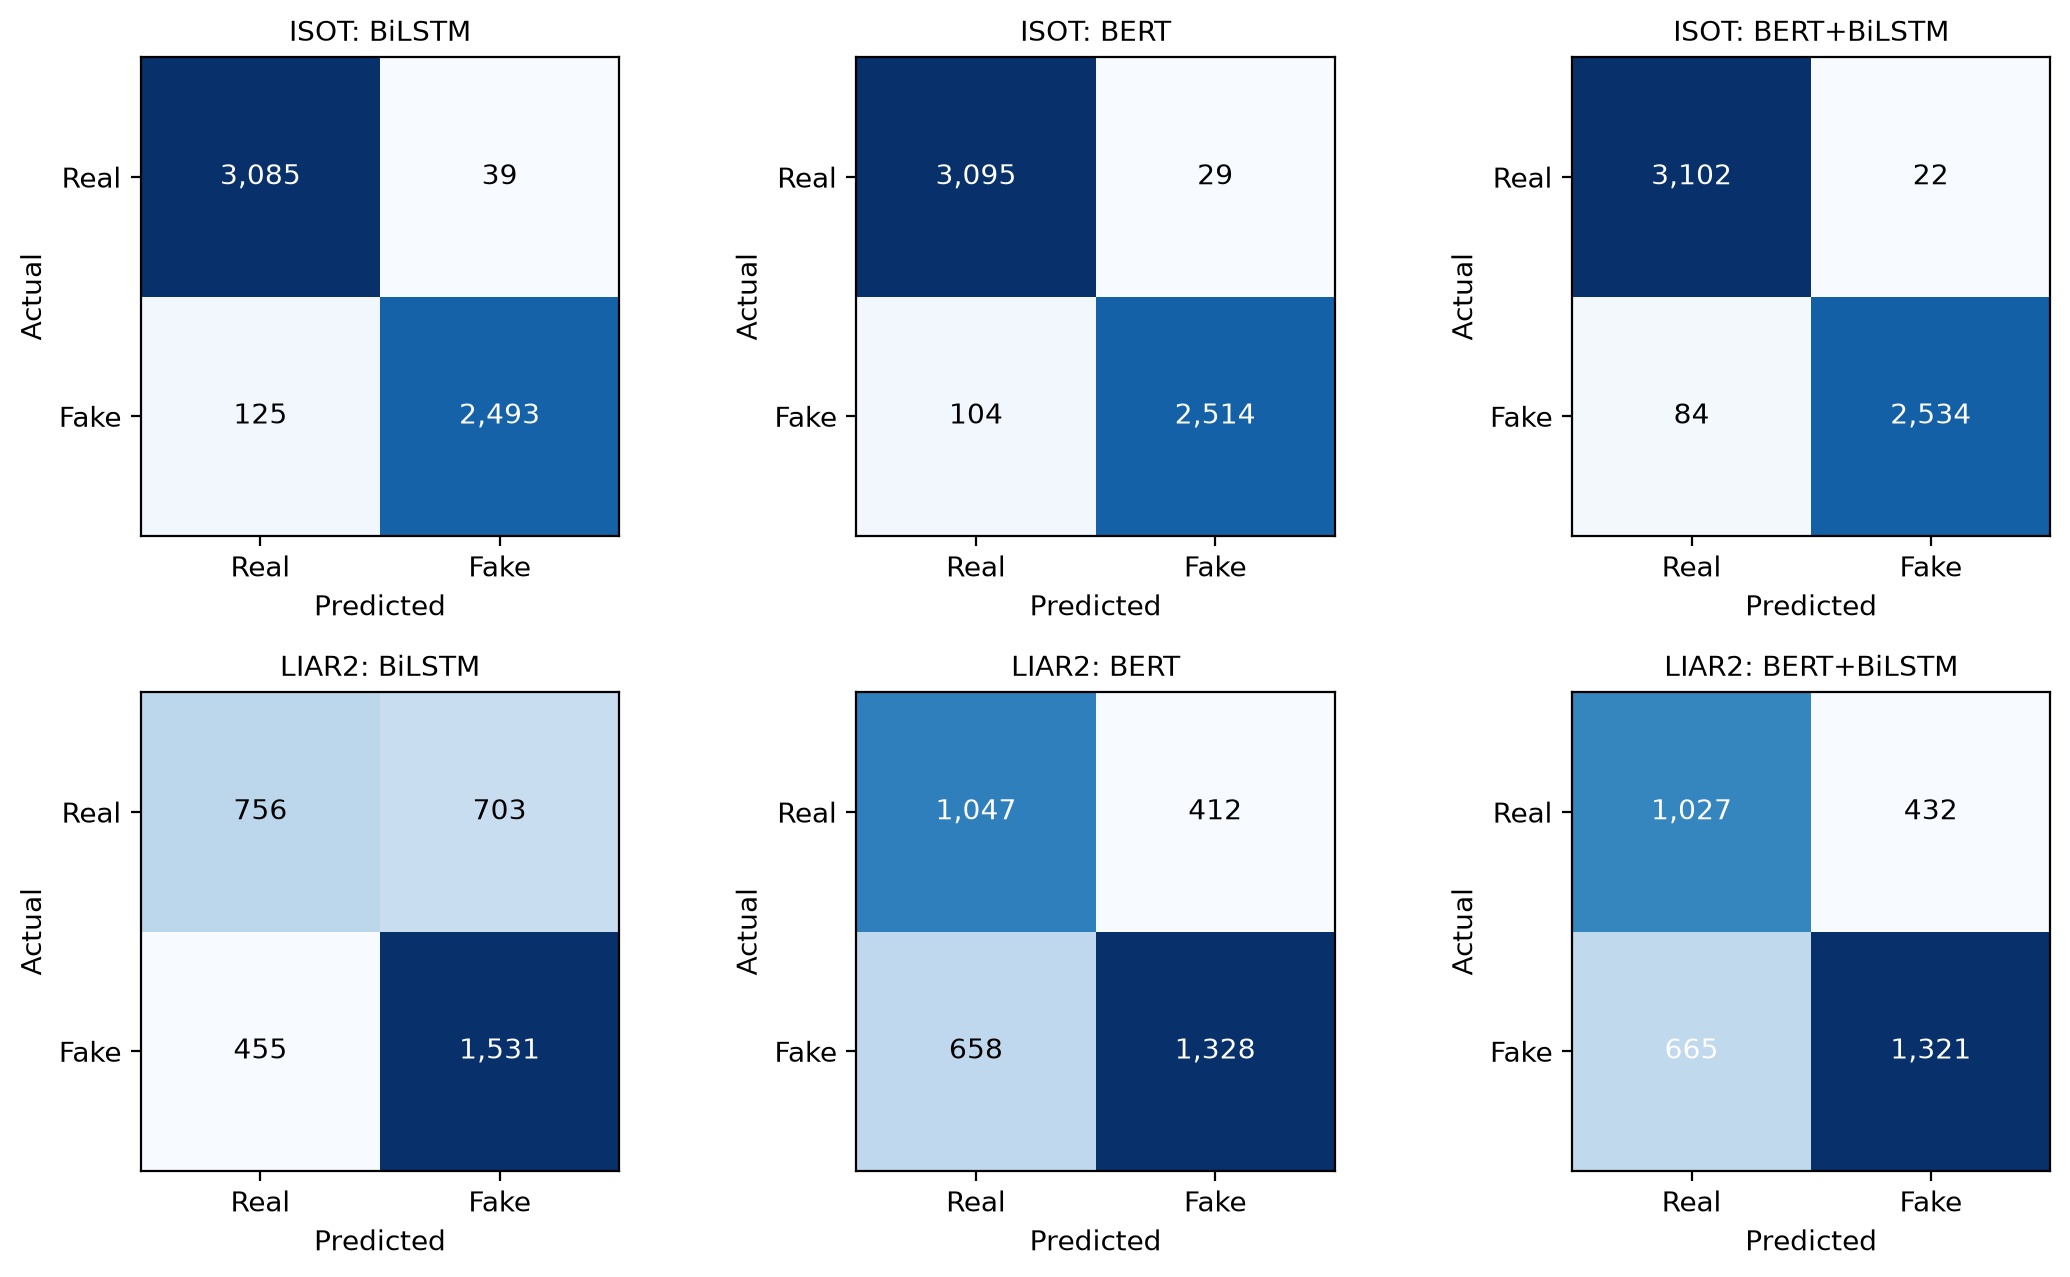
\includegraphics[scale=0.33]{Confusion.png}
\caption{Confusion Matrix for BERT, BiLSTM, and BERT+BiLSTM models across all datasets}
\label{fig:confusion}
\end{figure}

The ROC curve in Figure~\ref{fig:roc} plots the True Positive Rate against the False Positive Rate across classification thresholds; a curve closer to the top-left corner, and correspondingly a higher Area Under the Curve (AUC), indicates better discrimination between real and fake news.

\begin{figure}[h]
\centering
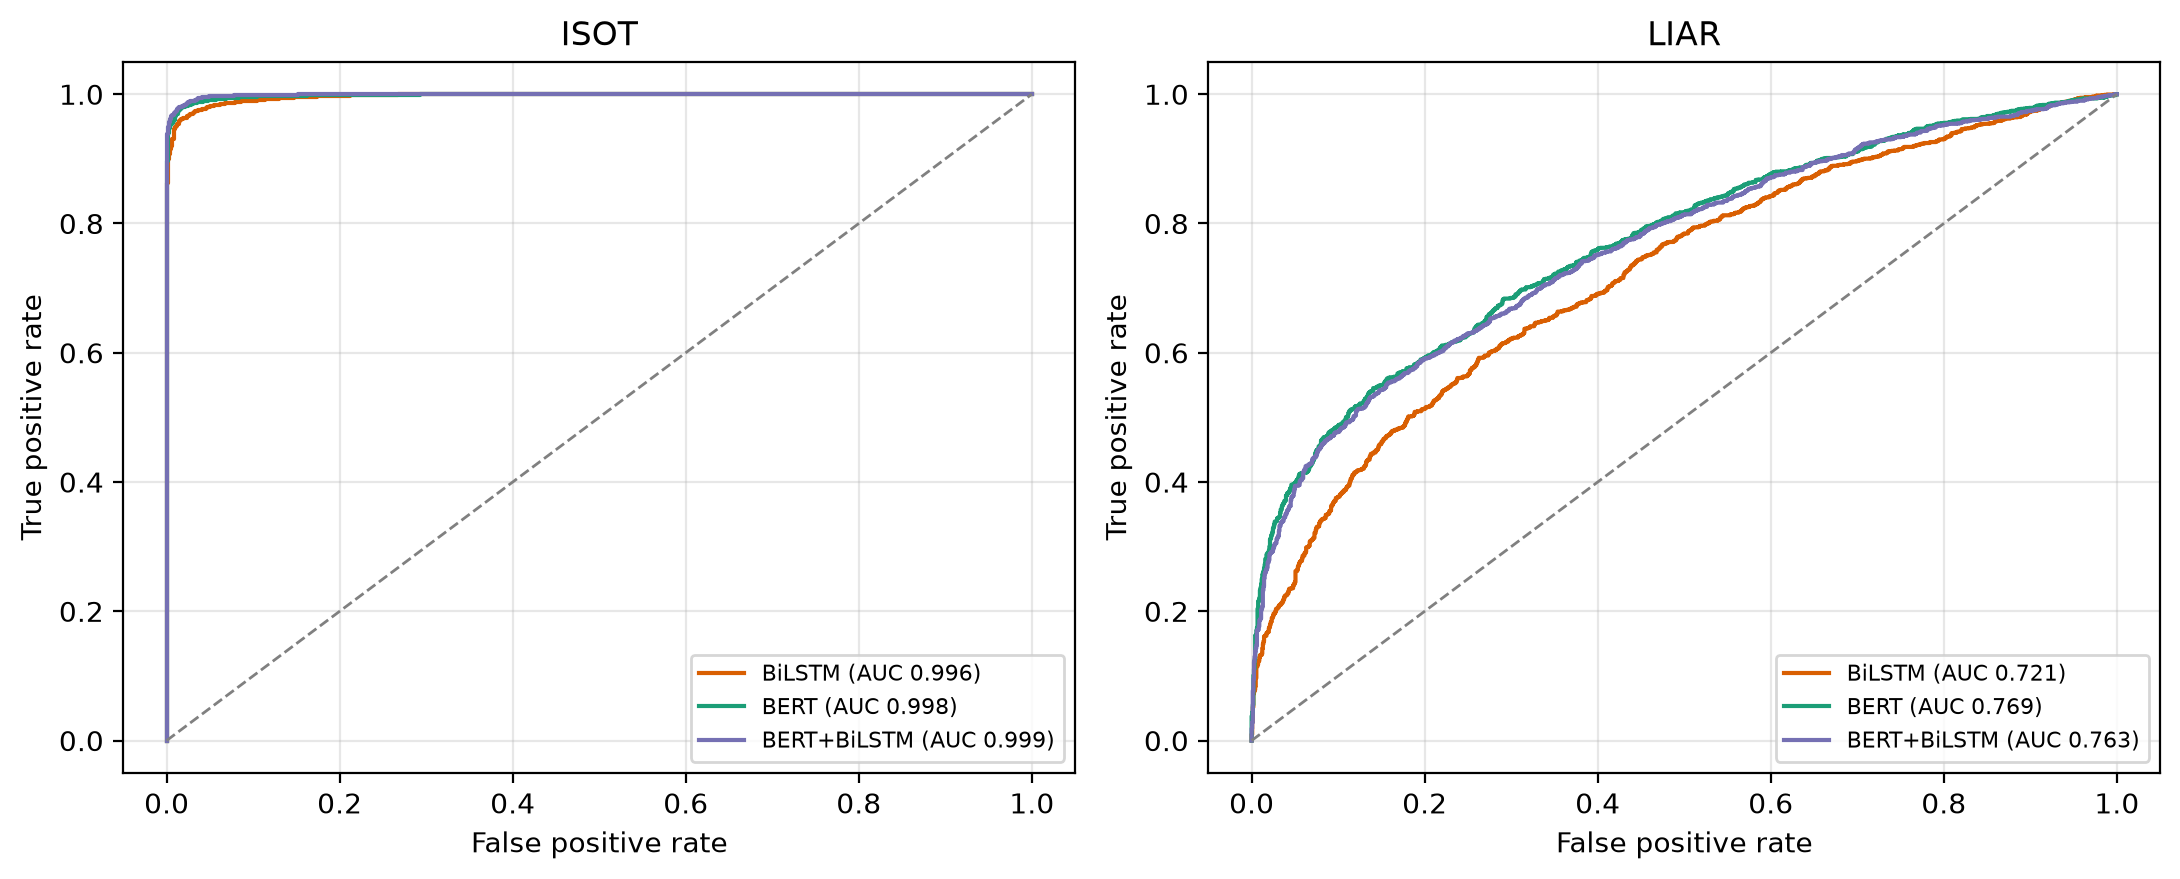
\includegraphics[scale=0.33]{ROC.png}
\caption{ROC Curves for BERT, BiLSTM, and BERT+BiLSTM models across all datasets}
\label{fig:roc}
\end{figure}

The precision--recall (PR) curve in Figure~\ref{fig:pr} shows the trade-off between precision and recall at different classification thresholds, which is particularly informative under class imbalance.

\begin{figure}[h]
\centering
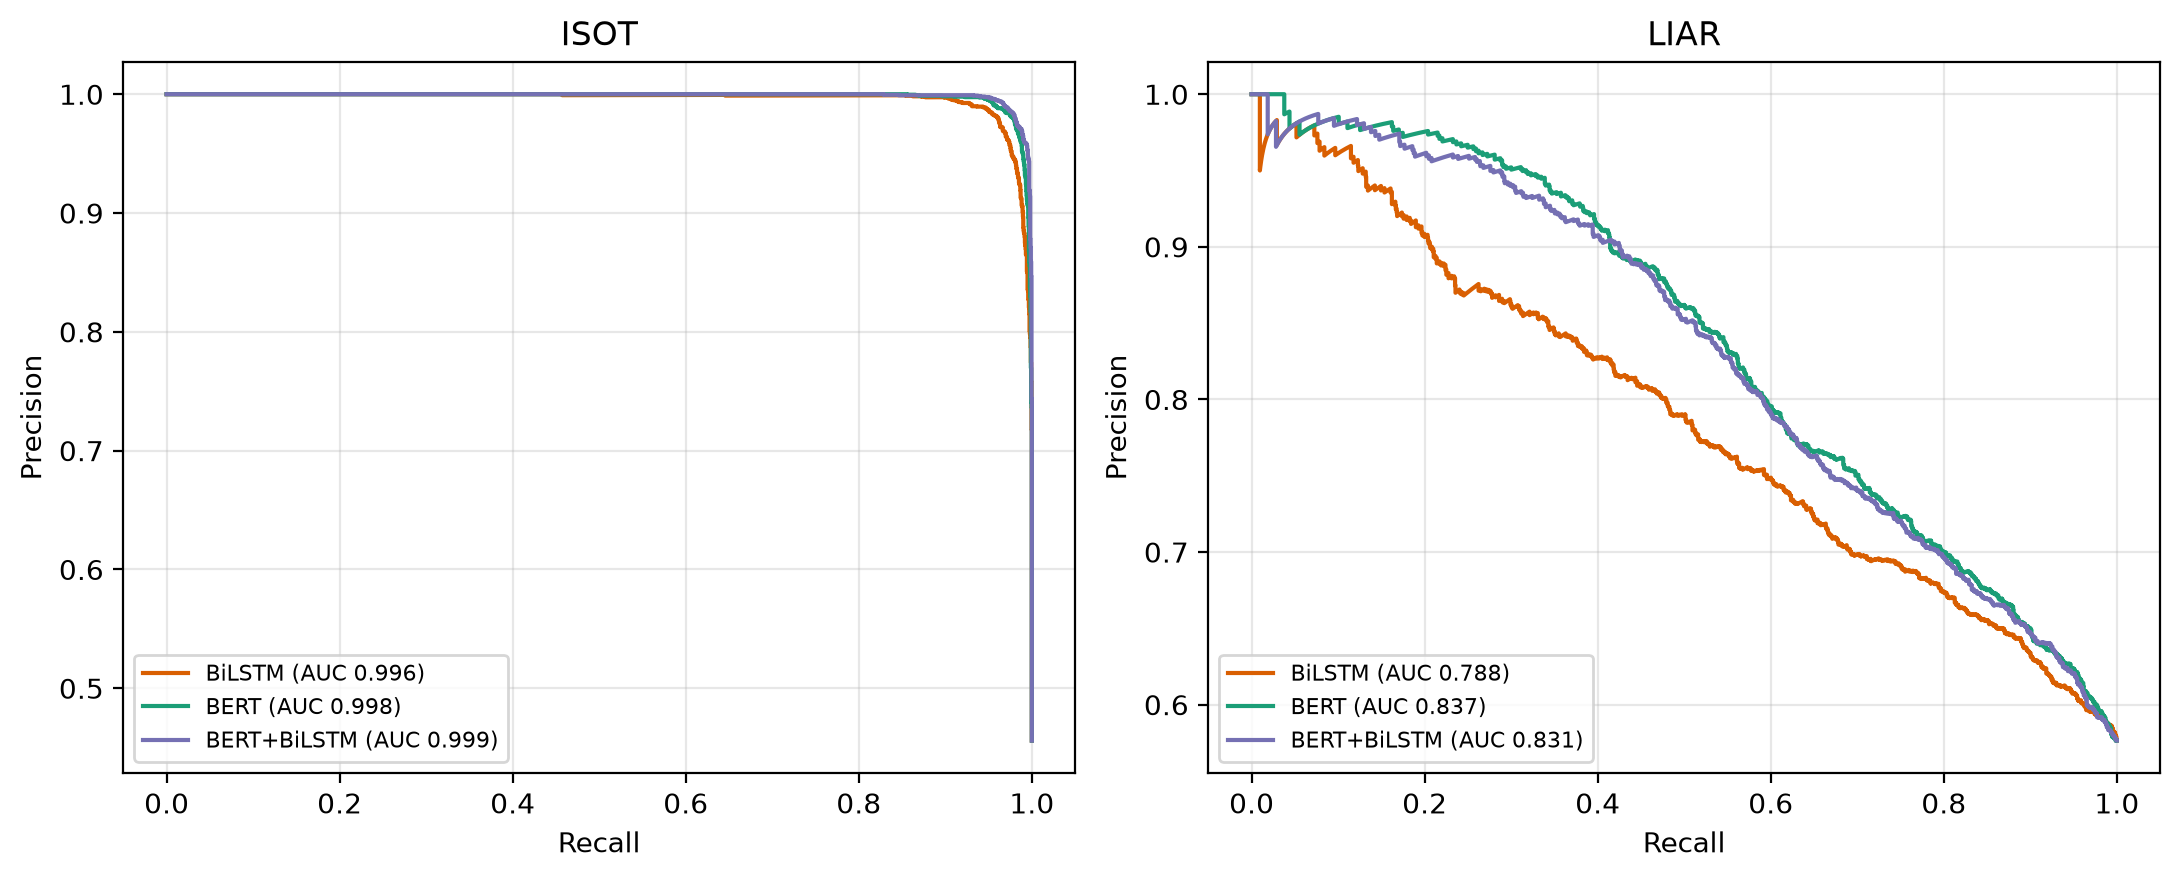
\includegraphics[scale=0.33]{PR_Curve.png}
\caption{Precision--Recall Curves for BERT, BiLSTM, and BERT+BiLSTM models across all datasets}
\label{fig:pr}
\end{figure}

Finally, the training/validation loss curves in Figure~\ref{fig:loss} show how each model's loss evolved over training epochs, indicating convergence behaviour and the degree of overfitting or underfitting.

\begin{figure}[h]
\centering
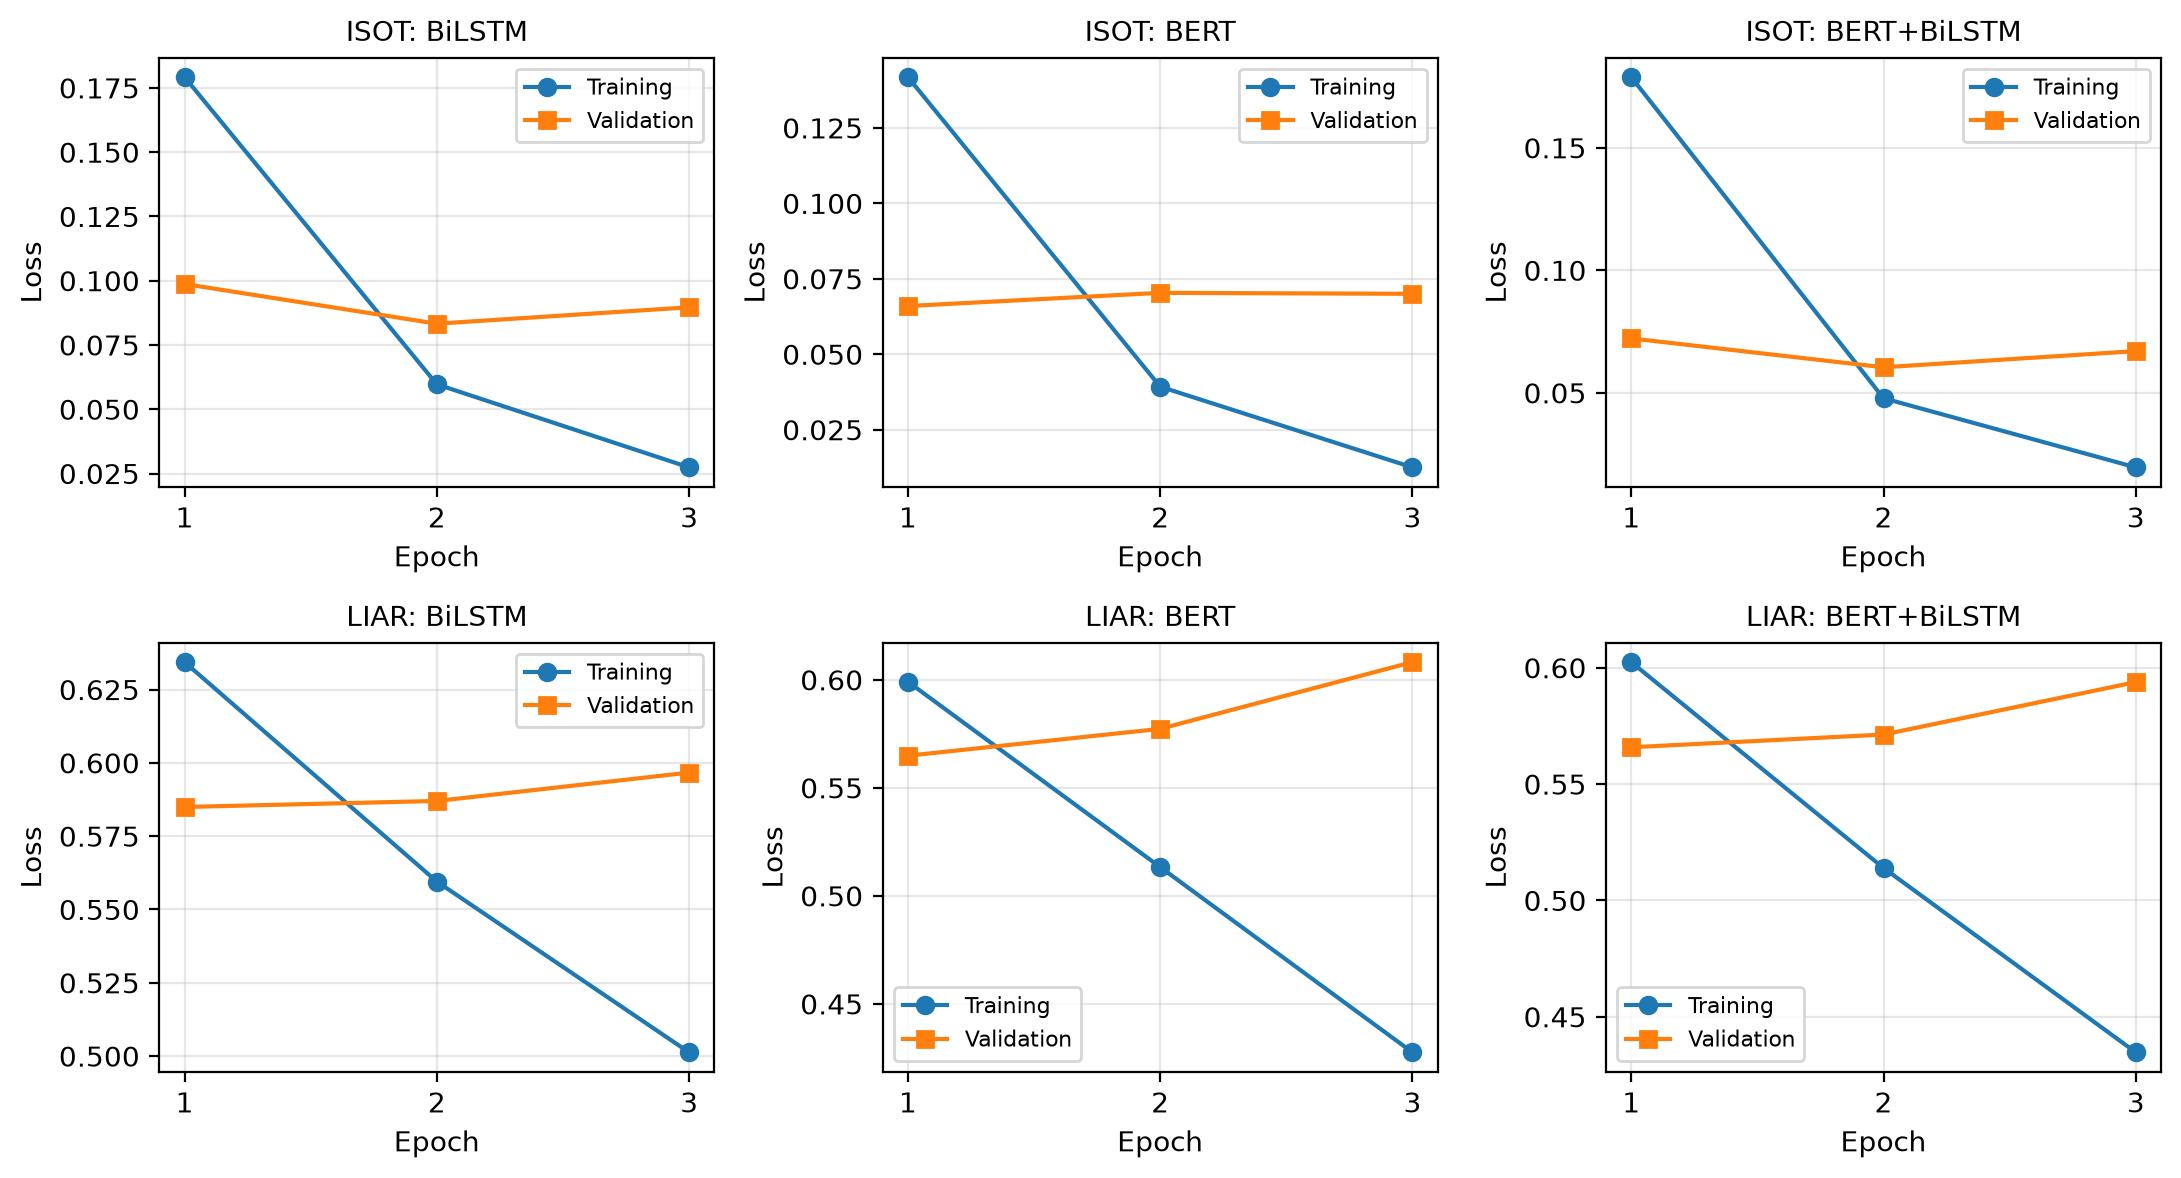
\includegraphics[scale=0.7]{Loss.jpg}
\caption{Loss Curves for BERT, BiLSTM, and BERT+BiLSTM models across all datasets}
\label{fig:loss}
\end{figure}

\subsection{Preliminary Zero-Shot Evaluation with a Local LLM}

To begin probing the LLM-based direction identified as future work in the conclusion chapter, a preliminary zero-shot experiment was conducted using a locally hosted large language model, rather than the fine-tuned BiLSTM/BERT/BERT+BiLSTM classifiers described above. The open-weight instruction-tuned model Qwen2.5-1.5B-Instruct \cite{Yang2024Qwen25} was run entirely on local CPU hardware via the Hugging Face \texttt{transformers} library \cite{Wolf2020Transformers}, with no fine-tuning, no retrieval augmentation, and no task-specific training of any kind. For each article, the model was given the headline and a truncated excerpt of the article body inside a system prompt instructing it to answer with exactly one word, REAL or FAKE, and its output was parsed and compared against the ground-truth label.

The evaluation was performed on a stratified random sample of 300 articles (150 real, 150 fake) drawn from the same ISOT-derived real/fake news corpus \cite{ISOTDataset} used elsewhere in this study, so that the results are directly comparable in kind, if not in scale, with Table \ref{tab:comparison}. Table \ref{tab:llm-comparison} reports the resulting metrics.

\begin{table}[H]
\centering
\caption{Zero-Shot Performance of a Local LLM Compared to Fine-Tuned Models}
\label{tab:llm-comparison}
\small
\begin{tabular}{|l|c|c|c|c|}
\hline
\textbf{Model} & \textbf{Accuracy} & \textbf{Precision} & \textbf{Recall} & \textbf{F1 Score} \\ \hline
BiLSTM (fine-tuned) & 0.5000 & 0.2500 & 0.5000 & 0.3333 \\
BERT (fine-tuned) & 0.9500 & 0.9545 & 0.9500 & 0.9499 \\
BERT + BiLSTM (fine-tuned) & 0.9500 & 0.9545 & 0.9500 & 0.9499 \\
Local LLM, Qwen2.5-1.5B-Instruct (zero-shot) & 0.7233 & 0.9136 & 0.4933 & 0.6407 \\ \hline
\end{tabular}
\end{table}

The zero-shot local LLM reaches 72.33\% accuracy without any task-specific training, which is well above a random baseline but clearly below the fine-tuned transformer models. Its precision (0.9136) is high, meaning that articles it flags as FAKE are usually genuinely fake, but its recall (0.4933) is comparatively low: the model fails to identify roughly half of the actual fake articles in the sample, instead defaulting to a REAL verdict when the writing style alone does not present an obvious red flag. This asymmetry is consistent with the model reasoning purely from surface linguistic style rather than from verified evidence, since well-written fabricated articles can be stylistically indistinguishable from genuine reporting without external fact-checking signals.

These preliminary results are consistent with, and directly motivate, the RAG-based direction already outlined in the Future Scope discussion below: grounding the LLM's classification in retrieved evidence from sources such as Snopes, PolitiFact, or Wikipedia, rather than relying on stylistic judgement alone, would be expected to particularly improve recall on subtler fake articles.

\subsection{GRU-Based Hybrid Architectures}

To examine whether lighter recurrent architectures can approach the transformer results, a standalone Gated Recurrent Unit (GRU) model and four GRU-based hybrids were trained on the ISOT-derived Kaggle corpus (23,481 fake and 21,417 real articles). Only the article headline was used as input. Headlines were lower-cased, stripped of non-alphanumeric characters and stopwords, tokenized with a 10,000-word vocabulary (12,000 for GRU+BiLSTM), and padded or truncated to 40 tokens. The data were split in a stratified 70:15:15 ratio, giving 31,428 training, 6,735 validation, and 6,735 test samples. All models were trained with the Adam optimizer (learning rate $10^{-3}$), binary cross-entropy loss, batch size 64, dropout 0.3, and at most 12 epochs, with early stopping on validation loss (patience 3, best weights restored).

The five architectures are: (i) a single GRU layer followed by global max-pooling over all time steps; (ii) GRU followed by an LSTM layer; (iii) a 1D convolution and pooling stage feeding a GRU; (iv) GRU followed by a Bidirectional LSTM; and (v) two 1D residual convolutional blocks feeding a GRU. Table \ref{tab:gru-comparison} reports the test-set results.

\begin{table}[H]
\centering
\caption{Test Performance of GRU and GRU-Hybrid Models (Headline-Only Input)}
\label{tab:gru-comparison}
\small
\begin{tabular}{|l|c|c|c|c|c|}
\hline
\textbf{Model} & \textbf{Loss} & \textbf{Accuracy} & \textbf{Precision} & \textbf{Recall} & \textbf{F1 Score} \\ \hline
GRU + BiLSTM & 0.1202 & 0.9546 & 0.9694 & 0.9429 & 0.9560 \\
GRU & 0.1249 & 0.9531 & 0.9596 & 0.9503 & 0.9549 \\
GRU + CNN & 0.1253 & 0.9534 & 0.9685 & 0.9415 & 0.9548 \\
GRU + LSTM & 0.1290 & 0.9520 & 0.9454 & 0.9640 & 0.9546 \\
GRU + ResNet & 0.1179 & 0.9513 & 0.9672 & 0.9387 & 0.9528 \\ \hline
\end{tabular}
\end{table}

\begin{figure}[htbp]
\centering
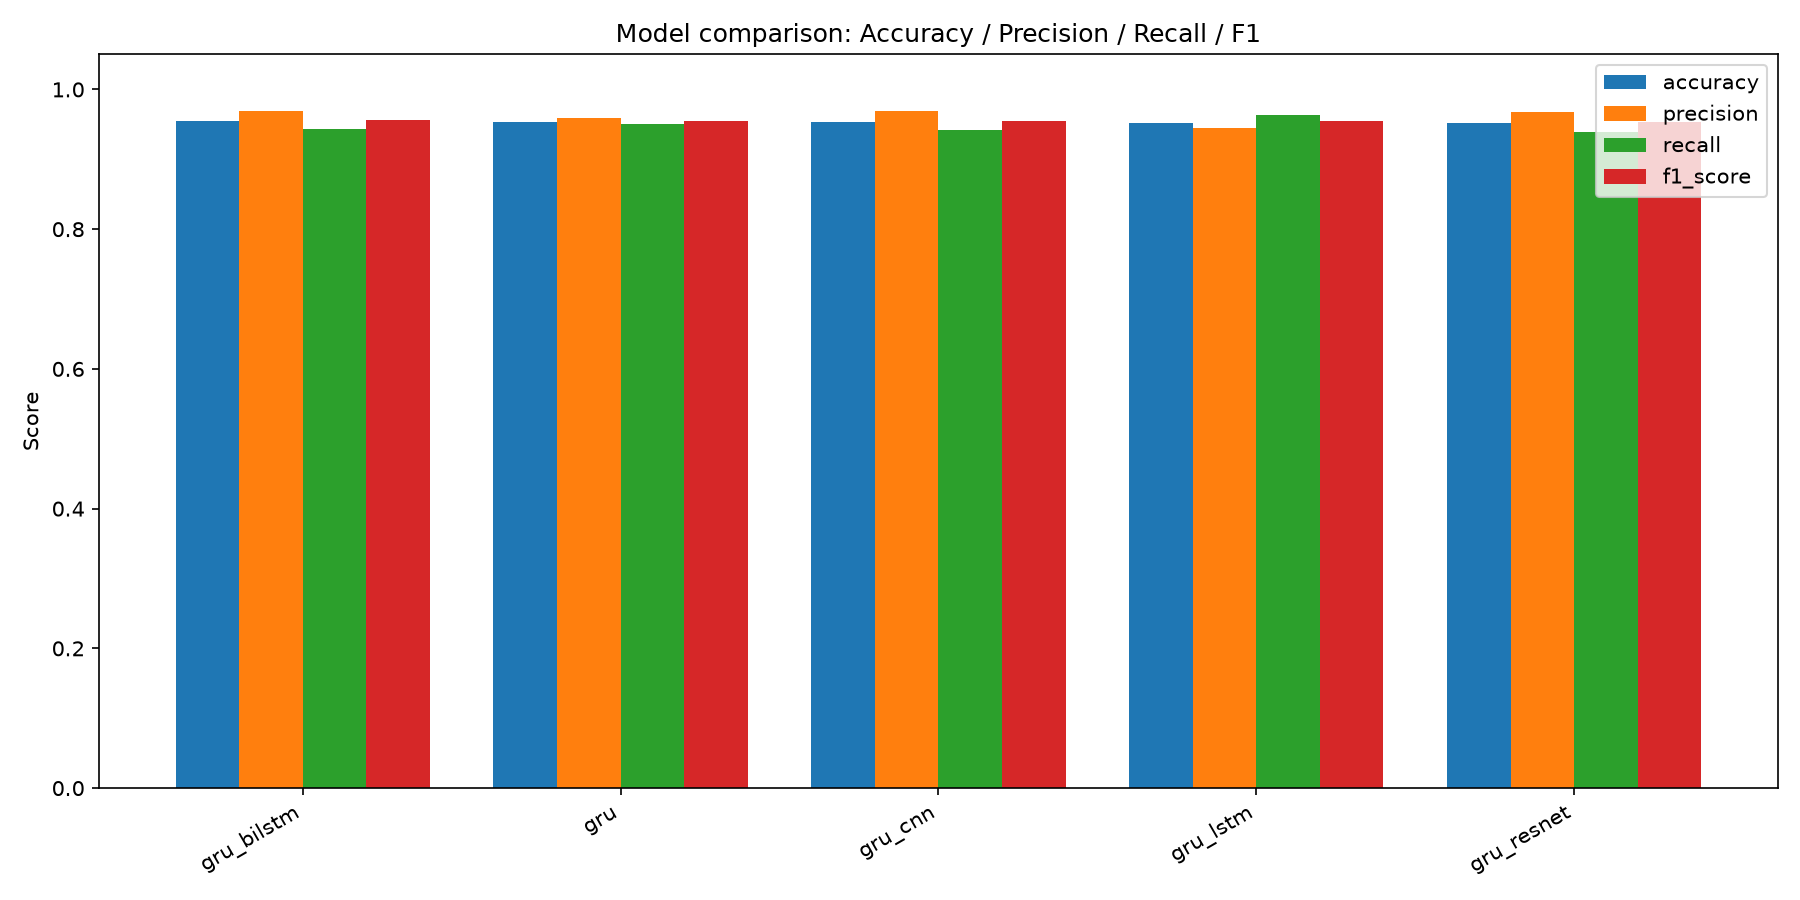
\includegraphics[width=0.88\textwidth]{./chap5-experimentalresults/comparison_metrics.png}
\caption{Accuracy, Precision, Recall and F1 Score of the GRU and GRU-Hybrid Models}
\label{fig:gru_metrics}
\end{figure}

All five models fall within 0.4 percentage points of each other in accuracy and 0.33 points in F1, so the added convolutional, residual, or second recurrent stage gives no meaningful gain over the standalone GRU. GRU+BiLSTM has the highest F1 (0.9560) and GRU+ResNet the lowest test loss (0.1179), but these differences are small. The hybrids trade precision against recall: GRU+BiLSTM has the highest precision (0.9694), while GRU+LSTM has the highest recall (0.9640). The standalone GRU collapsed to predicting the majority class when only its final hidden state was used; pooling over every time step resolved this. GRU+ResNet trained less stably, with validation accuracy dropping to 0.7526 at one epoch before recovering. These models, trained on short headlines with a small vocabulary, reach accuracy close to that of the fine-tuned BERT models in Table \ref{tab:comparison} with far smaller models.

\subsection{Cross-Dataset Generalization}
The in-domain scores above are measured on ISOT, whose headlines carry source artifacts such as the ``(Reuters)'' tag. To test whether the models learn the news content rather than these markers, we cleaned the source tags and URLs, removed duplicate titles, split each dataset 70/15/15 with stratification, and trained on one dataset while testing on the other. The second dataset is LIAR2, with labels 0--2 treated as fake and 3--5 as real. Every setting was repeated over three random seeds (five for the GRU), and Table \ref{tab:cross-dataset} reports the mean and standard deviation.

\begin{table}[htbp]
\centering
\caption{Cross-dataset results (mean $\pm$ std over seeds). Cross-domain rows use the full other dataset as the test set.}
\label{tab:cross-dataset}
\begin{tabular}{llllll}
\hline
Model & Train & Test & Accuracy & F1 & AUC \
\hline
GRU & ISOT & ISOT (in-domain) & 0.962 $\pm$ 0.001 & 0.958 $\pm$ 0.002 & 0.993 \
GRU & ISOT & LIAR2 (cross) & 0.532 $\pm$ 0.009 & 0.662 $\pm$ 0.013 & 0.466 \
GRU & LIAR2 & LIAR2 (in-domain) & 0.680 $\pm$ 0.006 & 0.725 $\pm$ 0.004 & 0.749 \
GRU & LIAR2 & ISOT (cross) & 0.475 $\pm$ 0.008 & 0.627 $\pm$ 0.004 & 0.681 \
BERT & ISOT & ISOT (in-domain) & 0.984 $\pm$ 0.002 & 0.982 $\pm$ 0.002 & 0.999 \
BERT & ISOT & LIAR2 (cross) & 0.504 $\pm$ 0.001 & 0.611 $\pm$ 0.001 & 0.472 \
BERT & LIAR2 & LIAR2 (in-domain) & 0.694 $\pm$ 0.004 & 0.733 $\pm$ 0.013 & 0.770 \
BERT & LIAR2 & ISOT (cross) & 0.460 $\pm$ 0.002 & 0.626 $\pm$ 0.001 & 0.562 \
BERT & ISOT + LIAR2 & ISOT (in-domain) & 0.984 $\pm$ 0.001 & 0.982 $\pm$ 0.001 & 0.998 \
BERT & ISOT + LIAR2 & LIAR2 (in-domain) & 0.693 $\pm$ 0.004 & 0.717 $\pm$ 0.009 & 0.772 \
\hline
\end{tabular}
\end{table}

Three findings follow. First, both models separate ISOT almost perfectly in-domain (BERT AUC 0.999) but fall to chance on LIAR2 (accuracy 0.50, AUC 0.47), and a model trained on LIAR2 falls below chance on ISOT. The high in-domain accuracy therefore reflects dataset-specific patterns more than transferable fake-news cues. Second, BERT gives only a small gain over the GRU on LIAR2 (F1 0.733 against 0.725), so a larger encoder does not by itself fix this. Third, training on both datasets keeps ISOT accuracy at 0.984 and LIAR2 AUC at 0.772, so mixing sources costs nothing in-domain, but we have not yet tested it on a third, unseen dataset. Closing the cross-domain gap is the main remaining work: stronger encoders, article-body input, retrieval-augmented classification, and explainability checks.

\section{Result Discussion}

The experimental outcomes show that the standalone BiLSTM architecture performed poorly on the primary dataset. Its precision, recall, and F1-score of 0.2500, 0.5000, and 0.3333 respectively indicate that it could not reliably distinguish fake news from real news, and its comparatively high final loss (0.6571) shows that the model failed to converge well within the training budget. This poor performance is best explained by the limited number of training epochs, the absence of extensive hyperparameter tuning, and the inherent complexity of the fake news classification task relative to the modelling capacity exercised here.

By contrast, the BERT model performed substantially better, achieving 95\% accuracy with a precision of 0.9545, a recall of 0.9500, and an F1-score of 0.9499. Its much lower final loss (0.0686) indicates good convergence and strong discriminative power, attributable to BERT's pre-trained, bidirectional contextual representations. The hybrid BERT + BiLSTM model performed essentially identically to standalone BERT -- 95\% accuracy, 0.9545 precision, 0.9500 recall, and an F1-score of 0.9499 -- despite a slightly higher final loss (0.0998). This demonstrates that, under the present training configuration, adding a BiLSTM layer on top of BERT neither meaningfully improves nor degrades performance.

The cross-dataset results in Table~\ref{tab:comparison_extended} confirm that these trends generalize: on both LIAR and ISOT, BiLSTM again underperforms substantially relative to BERT and BERT + BiLSTM, while the two transformer-based models remain closely matched to each other, indicating that transformer-based representations generalize consistently and reliably across datasets of different size, domain, and label distribution.

Despite the hybrid model's lack of measurable improvement over standalone BERT in this setting, these results should not be read as evidence that hybridization is without merit. The BiLSTM component in the hybrid model is layered on top of BERT's contextual embeddings specifically to capture additional sequential dependencies, a capability that may become more valuable with larger datasets, longer training schedules, and more extensive hyperparameter optimization -- conditions that were deliberately constrained in this study to keep the comparison tractable and fair across models. The visualizations in Figures~\ref{fig:confusion}--\ref{fig:loss} corroborate this discussion: BERT converges quickly with a small gap between training and validation loss (good generalization), BiLSTM converges slowly with a persistently higher loss (underfitting), and BERT + BiLSTM converges smoothly but without a clear advantage over BERT alone under the current setup.

\section{Summary}

This chapter presented the experimental setup, datasets, hyperparameters, and results used to evaluate the proposed fake news detection models. The standalone BiLSTM model underperformed significantly relative to the transformer-based models, while BERT and the hybrid BERT + BiLSTM model performed comparably well and generalized consistently across the LIAR and ISOT datasets. These findings, and their implications for future work, are discussed further in Chapter~5.
